\section{Numerical Tests}

\subsection{Cases Configuration}

The setup is shown in Fig. \ref{fg:config}, where the heavy (liquid) and light (gas) phases are represented with gray and white colors respectively. The distance $h$ between the cylinder top and the undisturbed free surface is taken as the measure of the cylinder submergence. Uniform inflow velocity with module $U$ is imposed on the inlet. The chosen Froude number based on the diameter of the cylinder $d$ is defined as
\begin{equation}
 Fr = \frac{U}{\sqrt{gd}}
\label{eq:froude}
\end{equation}
where $g$ is the gravity acceleration. Also, the Reynolds number based on the inlet velocity $U$ and the cylinder diameter $d$, is calculated as
\begin{equation}
 Re = \frac{\rho_l U d}{\mu_l}
\label{eq:reynolds}
\end{equation}
being $\rho_l,\mu_l$ the density and the dynamic viscosity of the heavier phase.

\begin{figure}[ht]
  \centering
  \includegraphics[width=0.9\columnwidth]{images_10thspheric/config.pdf}
  \caption{Case configuration, initial and boundary conditions.}
  \label{fg:config}
\end{figure}

In the reference work of Reichl et.al \cite{Reichl05}, densities and viscosities ratios are established in $\rho_l/\rho_g = \mu_l/\mu_g=100$ in order to avoid convergence problems. PFEM-2 method does not suffer from these drawbacks, allowing more realistic water-air ratios. However, the original ratios are employed to guarantee same simulation conditions. Regarding the boundary conditions, a uniform flow with velocity $U$ is imposed at the inlet boundary, and typical FEM natural boundary condition is used for the top and outflow boundaries. The floor of the channel and the cylinder surface are considered as no-slip walls.

Flow conditions are inspirated in the work of Bouscasse \cite{Bouscasse14} which investigates the flow behavior employing a range of Froude numbers ($Fr=0.3$, $0.6$, $0.8$, $1.2$, $1.6$ and $2.0$) for a fixed submergence ratio ($h/d=0.55$) and a fixed Reynolds number of $Re=\frac{\rho_l U d}{\mu_l}=180$.

As it was explained in the introduction, one of the advantages of using SPH as numerical method allowing is to treat larger fragmentation of the free surface, when compared to FLUENT-VOF technique used by Reichl and colleagues. The PFEM-2 method employed in the current work, since its particle nature, is also able to treat large deformations and breakups, but, due to the use of the temporal integrator named XIV-S \cite{Idelsohn12}, it can manage larger time steps resulting in shorter computing times \cite{Gimenez2015186}. PFEM-2 simulations were carried out employing the implementation presented in \cite{Gimenez14}.



\subsection{Simulation Results}

Figure \ref{fg:vort_Re180} shows the influence of the Froude number in the flow characteristics, represented by the dimensionless vorticity. When the lowest Froude number is imposed $Fr=0.3$, the free-surface deforms very little being similar to a no-slip wall where the vortex production presents similar distribution to the only one-phase tests \cite{PRICE2002175}. As the Froude number increases $Fr=0.6$, the physics changes drastically. Although the free-surface just deforms in the proximities of the cylinder, the vortex advection is completely blocked. Another important observation is that, a recirculation area appears just behind the cylinder and close to the free-surface, the positive vorticity generated at the free surface by the spilling breaker builds up a large positive meta-vortex behind the cylinder which is then advected downstream. Reaching intermediate-high Froude numbers (1.2 and 1.6) structures developed are not periodic, while as the vortex production remains blocked due to the continuous breakups occurring at free-surface. Although the non-stationary behavior of the flow at free-surface, this phenomena allows to obtain constant forces acting over the cylinder. Analysis and discussions presented in this paragraph are in agreement with the work of Bouscasse et. al \cite{Bouscasse14}.

When the analysis for $Fr=2.0$ is done, differences between the flow characteristics of Bouscasse et. al \cite{Bouscasse14} and the present work are found. Bouscasse shows that at this Froude number the vortex shedding is recovered while the current results find instabilities but not shedding. In order to present a regime where a structure similar to a Von Karman street appears, a case with $Fr=3.5$ was also run finding vortex shedding behind the cylinder and large distortions of the free-surface but without the characteristic chaos of the intermediate Froude numbers. In order to confirm if there is any dependence between the Froude number and the transition from a convective to an absolute instability in the cylinder flow, next section will present a stability analysis study using the Froude number as the principal parameter.


\begin{figure}[htbp]
  \begin{center}
    \subfloat[$Fr=0.3$]{
	  \label{fg:vort_a}
	  \includegraphics[width=.9\columnwidth]{images_10thspheric/Fr_0_3_Re_180_h_0_55_vorticity.png}
    } \\
\subfloat[$Fr=0.6$]{
	  \label{fg:vort_b}
	  \includegraphics[width=.9\columnwidth]{images_10thspheric/Fr_0_6_Re_180_h_0_55_vorticity.png}
    } \\
% \subfloat[$Fr=0.8$]{
% 	  \label{fg:vort_c}
% 	  \includegraphics[width=.9\columnwidth]{images_10thspheric/Fr_0_8_Re_180_h_0_55_vorticity.png}
%     } \\
\subfloat[$Fr=1.2$]{
	  \label{fg:vort_d}
	  \includegraphics[width=.9\columnwidth]{images_10thspheric/Fr_1_2_Re_180_h_0_55_vorticity.png}
    } \\
\subfloat[$Fr=1.6$]{
	  \label{fg:vort_e}
	  \includegraphics[width=.9\columnwidth]{images_10thspheric/Fr_1_6_Re_180_h_0_55_vorticity.png}
    } \\
\subfloat[$Fr=2.0$]{
	  \label{fg:vort_f}
	  \includegraphics[width=.9\columnwidth]{images_10thspheric/Fr_2_0_Re_180_h_0_55_vorticity.png}
    } \\
\subfloat[$Fr=3.5$]{
	  \label{fg:vort_g}
	  \includegraphics[width=.9\columnwidth]{images_10thspheric/Fr_3_5_Re_180_h_0_55_vorticity.png}
    } \\
  \end{center}
  \caption{Influence of Froude number on dimensionless vorticity $\hat\omega = curl(\vv) \sqrt{d/g}$ (scales from -3 (blue) to 3 (red)) with $h/d = 0.55$ and $Re=180$. Captures at $t^*=80$.
}
\label{fg:vort_Re180} 
\end{figure}


A summary of computed force coefficients can be seen in Fig. \ref{fg:CdCl}. The drag coefficient, calculated as $Cd=2 F_x/(\rho_l U^2 d)$ where $F_x=\mathbf{F} \cdot \mathbf{i}$ being $\mathbf{F}$ the force over the cylinder, decreases as the Froude number increases. A maximum lift $Cl=2 F_y/(\rho_l U^2 d)$ (in absolute value) is found at $Fr = 0.8$, and then a gentle monotonic reduction for the largest Froude number cases occurs. At each case, the drag and lift coefficients represent the temporal average for the computed case, and the bars shows the periodic variability of the amplitude. Only in the cases where the vortex shedding is not blocked, appreciable amplitude variation can be observed. Mean values and the majority of the amplitude variations present good agreement with the referenced work.

\begin{figure}[ht]
  \centering
  %%----primera subfigura----
  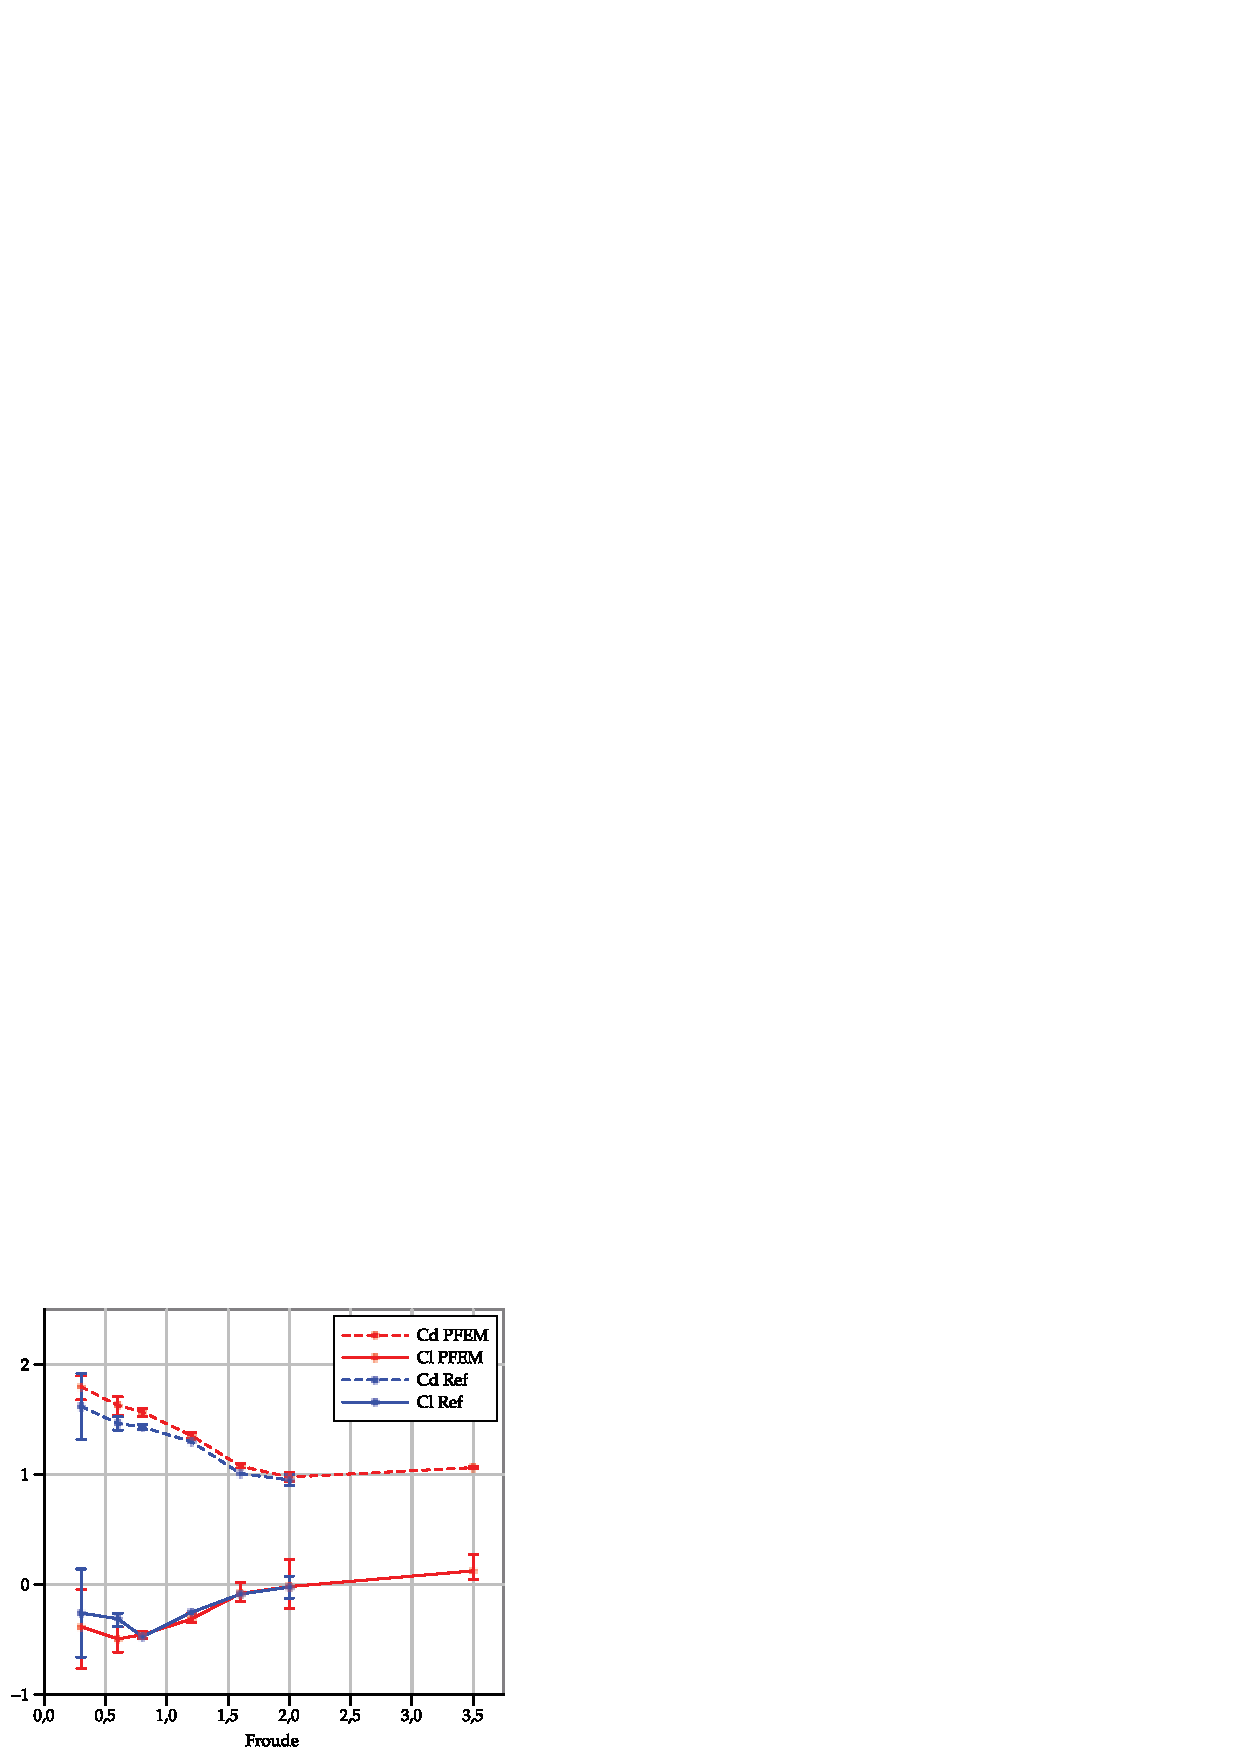
\includegraphics[width=0.95\columnwidth]{images_10thspheric/CdCl_Re180_hd_0_55.pdf}
  \caption{Drag and Lift coefficients calculated with PFEM-2 compared with the reference work of Bouscasse \cite{Bouscasse14}. $Re=180$.} %, $t^*=tU/d$. }
  \label{fg:CdCl}
\end{figure} 

\subsection{DMD-Analysis Results}



\begin{figure}[ht]
  \centering
  %%----primera subfigura----
  \includegraphics[width=0.95\columnwidth]{images_10thspheric/modos2.jpeg}
  \caption{Spectrum obtained after the DMD analysis when (for example 40 snapshot of one oscillating period were analyzed)using at $Fr=3.5$ $Re=180$.} 
  \label{fg:CdCl}
\end{figure} 

\begin{figure}[ht]
  \centering
  %%----primera subfigura----
  \includegraphics[width=0.95\columnwidth]{images_10thspheric/modos3.jpeg}
  \caption{Perturbation components of the most unstable mode obtained after the DMD analysis when (for example 40 snapshot of one oscillating period were analyzed)using at $Fr=3.5$ $Re=180$.}
  \label{fg:CdCl}
\end{figure} 



\begin{figure}[ht]
  \centering
  %%----primera subfigura----
  \includegraphics[width=0.95\columnwidth]{images_10thspheric/7vs40vslongersnaps.jpg}
  \caption{Drag and Lift coefficients calculated with PFEM-2 compared with the reference work of Bouscasse \cite{Bouscasse14}. $Re=180$.} %, $t^*=tU/d$. }
  \label{fg:CdCl}
\end{figure} 